\documentclass{article}


\usepackage{authblk}
\usepackage[T1]{fontenc}
\usepackage{indentfirst}
\usepackage{graphicx}
\usepackage{amsmath}
\usepackage{caption}
\usepackage{hyperref}
\usepackage{float}
\usepackage{subcaption}


\begin{document}

\title{Photoluminescence}
\author[1]{Woojin Han}
\affil[1]{Seoul National University, Seoul 151-747, Korea}
\maketitle
\begin{abstract}

\end{abstract}

\section{Introduction}
 In this experiment, photoluminescence(PL) of ruby and rhodamine 590 is measured.
 Analysis between PL peak statics of ruby and temperature is obtained.(\ref{result:temperature_peak_statics})
 The effect by aperture of spectrograph to PL result is declared, and proved.(\ref{result:aperture_effect})
 According to the peak intensity ratio, the mole ratio of $Cr^{3+}$ ion in the ruby is calculated.
 The apparatus data (\cite{ruby_spec}) is also found and compared to the calculation.


\subsection{Photoluminescence : General Theory}
 \label{intro:pl_general_theory}
 Photoluminescence is explained by two different parts, absortion and emission of light.
 Both events occur by the electronic transition through states, embedding the nature of the condensed matter.
 Therefore, the photoluminescence result lead us to measure the band diagram of the crystal.
 Not only the energy level of each band but also lifetime or exact orbital can be measured by the peak statics, such as peak width or intensity ratio.
 \begin{figure}[ht]
    \centering
    \begin{subfigure}[b]{6cm}
        \centering
        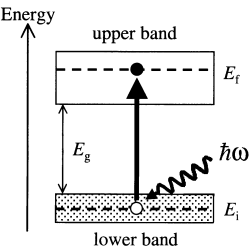
\includegraphics[width=4cm]{../results/intro_energy_absortion.png}
        \caption{}
    \end{subfigure}
    \hfill
    \begin{subfigure}[b]{6cm}
        \centering
        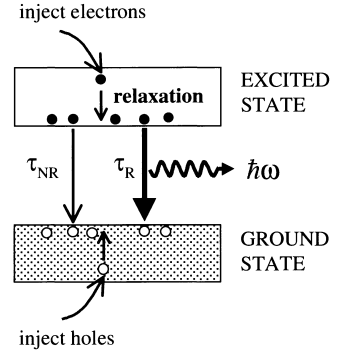
\includegraphics[width=4cm]{../results/intro_energy_emission.png}
        \caption{}
    \end{subfigure}
    \hfill
    \caption{Schematic diagram of (a)light absortion (b)light emission \cite{condensed_matter_optics}}
    \label{fig:pl_intro}
 \end{figure}

 \begin{figure}[ht]
    \centering
    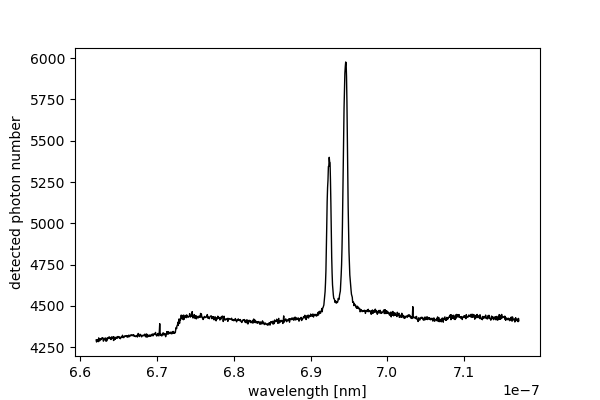
\includegraphics[width=8cm]{../results/Ruby(170.0)_raw_fig.png}
    \caption{photoluminescence results of Ruby in $170.0K$}
    \label{fig:pl_sample}
 \end{figure}
 Fig. \ref{fig:pl_intro}(a) shows the band diagram explaination of light absortion, creating hole in lower band transite to upper band.
 Fig. \ref{fig:pl_intro}(b) is the schematic diagram of light emission, slowly relaxing and emitting light while energy drops between band gap.
 Fig. \ref{fig:pl_sample} is one of the photoluminescence results in this experiment.
 The absorbed light was $532nm$, but we can find out the emitted light have wavelength around $690nm$.
 We can sure the electronic transition is the key mechanisms since the wavelength change can not be explained by scattering, especially for the peak nature.
 Therefore, the peak position is specific to the crystal structure or the molecular shapes.
 But the peak width have two reasons, natural and optical broadening. (\cite{quantum_optics})
 Natural broadening is intrinsic to the transition, caused by lifetime of the states.
 For lifetime $\tau$, the spectral function follows Lorentzian like equation (\ref{equation:natural_broadening}), $\omega$ is the angular frequency of light, and $\Delta \omega$ is full width at half maximum(FWHM) value which is related with lifetime.
 \begin{equation}
   g(\omega) = \frac{\Delta \omega}{2 \pi} \frac{1}{(\omega-\omega_0)^2 + (\Delta \omega/2)^2},\, \Delta \omega = \frac{1}{\tau}
   \label{equation:natural_broadening}
 \end{equation}
 And by the spectral effects by spectroscopy itself, the Gaussian shape optical broadening is inevitable.
 Therefore, I assume that the detected photoluminescence spectroscopy data will follow Voigt profile, which is a convolution results of Lorentzian and Gaussian function.


 \subsection{Ruby}
 \label{intro:ruby}
 In the theory of solid state luminescence, simultaneous emission is allowed between special states.
 Otherwise, electron can loses its energy in phonon which we call nonradiative transition.
 The phonon physics is explained by debye model, assuming that the highest frequency of phonon is restricted by the size of the lattice denoted as $\omega_D$.
 And phonon follows boson statics, can easily induces the density of states.
 
 \begin{multline}
  H= \sum_{n=0}^3 \epsilon_n \psi_n^\dagger \psi_n + \sum_k (\hbar \nu k) (a_k a_k^\dagger + \frac{1}{2}) + S_0 (C_{12} \psi_1^\dagger + \sum_{n=1,2} C_{n3} \psi_n^\dagger \psi_3 + c.c.) \\
   + S_0^2 (\sum_{n=0}^2 d_n \psi_n^\dagger \psi_n + [d_{12}\psi_1^\dagger \psi_2 + c.c.])
  \label{equation:phenomenological_hamiltonian}
 \end{multline}

 In \cite{Ruby_temp_theoretical}, they declare the phenomenological Hamiltonian of impurity ruby as equation \ref{equation:phenomenological_hamiltonian}.
 As the two big peak is observed near $690nm$, we assume three excited-state levels $n=1,2,3$ have energy of $\epsilon_1, \epsilon_2, \epsilon_3$ and wave function of $\psi_1, \psi_2, \psi_3$ respectivly.
 The first term is about the impurity electronic states energy.
 The second term is phonon energy, which $k$ is bounded by Debye frequency.
 In ruby, first and second excited states are $E_2$ levels and the photoluminescence peak appears by the spontaneous emission through $1\rightarrow0$ and $2\rightarrow0$.
 Empirically, $0=\epsilon_0<<\epsilon_1 < \epsilon_2 << \epsilon_3$, since the gren laser excites electron by $0\rightarrow3$ and by nonradiative $3\rightarrow1,2$ transition occurs.
 The leftover terms are suggested perturbation term in \cite{Ruby_temp_theoretical}, assuming the dopped $Cr^{3+}$ locates isotropic in enlarged Debye-model.
 In this experiment, the dopped ratio is small enough to fit in the assumption.
 \begin{multline}
  \epsilon_n (T) = \epsilon_n (0) + \alpha_n (\frac{T}{T_D})^4 \int_{0}^{T_D / T} dx \frac{x^3}{e^x -1} - \beta_{12} (-1)^n \frac{T_e}{T_D} (\frac{T}{T_D})^2 \\
  \times \int^{T_D/T}_{0} dx \frac{x^3}{e^x -1} \frac{P}{x^2 - (T_e/T_D)^2}
  \label{equation:peak_position}
 \end{multline}
 \begin{multline}
  \Gamma_n(T) = \Gamma_n(0) + \bar{\alpha_n} (\frac{T}{T_D})^7 \int^{T_D/T}_{0} dx \frac{x^6 e^x}{(e^x -1)^2}\\ + \pi \beta_{12} (\frac{T_e}{T_D})^3 [\delta_{n2}+\frac{1}{e^{T_e/T}-1}]
  \label{equation:peak_width}
 \end{multline}
 After calculating lowest order of perturbation theory, we have the peak position in function of temperature as equation \ref{equation:peak_position}.
 $T_D$ is Debye temperature, $\alpha_n , \beta_{12}$ is fitting coefficients, $T_e=(\epsilon_2 - \epsilon_1)/k_B$ is $42K$ in ruby.
 Equation \ref{equation:peak_width} shows the temperature dependance of each peak width, $\Gamma$ denotes the parameter of Lorentzian lineshape.
 $\bar{\alpha_n}$ is also a fitting variable, which have direct expression to hamiltonian coefficients.
 The first temperature perturbed term starting with $\alpha_n, \bar{\alpha_n}$ in both equation is a calculation of nonradiative effects.
 The second term starting with $\beta_{12}$ is the term of internal conversion between state $1,2$.
 In this case, the internal conversion can be disregarded, $\beta_{12}=0$.
 Specific fitting method and results in this experiment are denoted below. (\ref{result:temperature_peak_statics})

 Those explaination doesn't imply the specific states, since we never comes out with the crystal environments.
 Ruby is dopped crystal which basic structure is built by $Al_2O_3$, hexagonal crystal structure, $Cr^{3+}$ located in octahedral site.
 In this case both crystal and ion energy state affect themselves to have broad band structure or energy splits.
 $Al_2 O_3$ doesn't have any fluorescence bandgaps, since we can never find photoluminescence peaks on other dopped ions.
 Which means that the affected $Cr^{3+}$ energy structure is the key of this luminescence effects.
 Fig \ref{fig:ruby_band_structure}, adapted from \cite{Ruby_band_structure} shows the shift of ioninc energy structure.
 The left side of the diagram is the original orbital energy of free $Cr^{3+}$.
 As the cubic field parameter $Dq/B$ increases, the energy level splitted and broadened.
 The diagram at $Dq/B=3$ represents energy level of the $Cr^{3+}$ in ruby, which doesn't splitted enough and considered as constant.
 So, $^4A_2 , ^2E, ^2T_1 , ^4T_2$ is the $\epsilon_0, \epsilon_1, \epsilon_2, \epsilon_3$ state respectivly as explained.
 As a conclusion, the dopped ruby absorb green light to transite electron from $^4A_2 \rightarrow ^4T_2$ and nonradiative transite to $^4T_2 \rightarrow ^2T_1 , ^2E$ and give $R_1 , R_2$ emitted light peak by $^2T_1 , ^2E \rightarrow ^4A_2$. 

 \begin{figure}[ht]
  \centering
  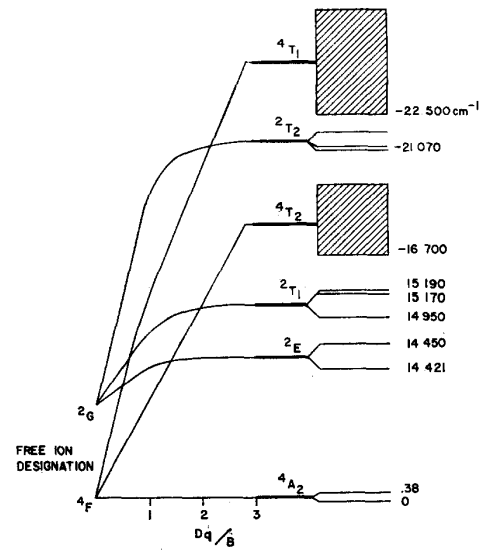
\includegraphics[width=6cm]{../results/ruby_band_diagram.png}
  \caption{Energy level diagram of $Cr^{3+}$ in ruby. adapted form \cite{Ruby_band_structure}}
  \label{fig:ruby_band_structure}
\end{figure}


\subsection{Rhodamine 6G(R6G)}
 Rhodamine 6G (R6G) is one of the highly fluorescent triarylmethane dyes.
 Fig. \ref{fig:rhodamine_structure} shows the molecular structure of R6G.
 It has three benzene ring, which allows each atomic orbital forms fluorescence cojugated system.
 In photochemistry, we assumes the linear combination of each atomic orbitals form molecular orbital.
 Which means that, the total hamiltonian of molecule is described by the function of linear coefficients.
 Therefore, eigenstate of the hamiltonian gives the energy diagram of a molecule.
 \begin{figure}[ht]
  \centering
  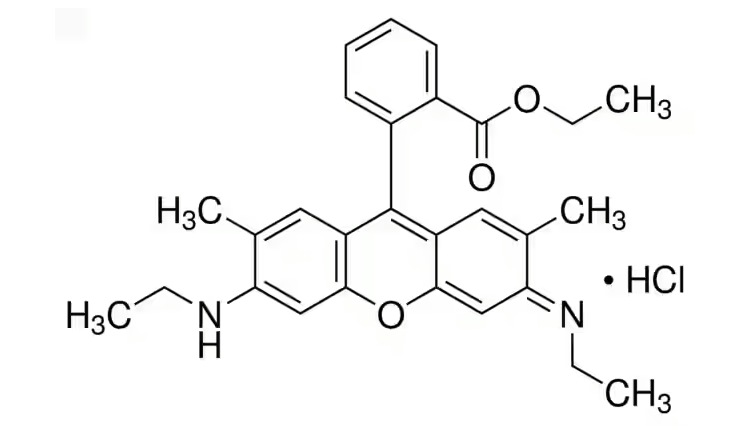
\includegraphics[width=6cm]{../results/Rhodamin_structure.png}
  \caption{Structural formula of R6G, adapted from \cite{rhodamine_sigma_aldrich}}
  \label{fig:rhodamine_structure}
 \end{figure}
 In this experiment, we dissolve R6G in ethylene glycol, which need different approach to ruby.
 Since the molecules does not fixed by its position, it can freely vibrate and rotate.
 Therfore, the PL results of R6G must consider a Raman shift.
 And also \cite{Rhodamine_dimer} reports that the concentration of the solution effects the peak position and FWHM.
 It declares a significant role of dimer formation by $\pi -\pi$ stacking interaction.
 But by Frank condon principle, the molecular position does not change while electric transition occurs, the energy gap between monomer and dimer is disregarded.

 \begin{figure}[ht]
  \centering
  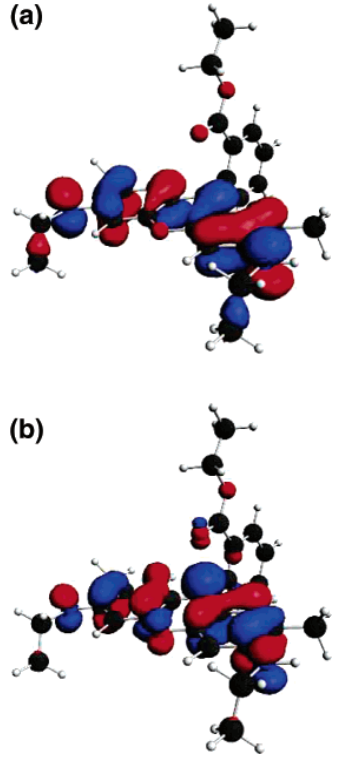
\includegraphics[width=4cm]{../results/Rhodamine_homo_lumo.png}
  \caption{The HOMO (a) and LUMO (b) of R6G adapted from \cite{rhodamine_HOMO_LUMO}}
  \label{fig:rhodamine_homo_lumo}
 \end{figure}

 In photochemistry the nonradiative, and radiative transition can be explained once in Jablonski diagram.
 Jablonski diagram have each vibrational modes in multiplicity of states, denoted by $M = 2S+1$. $S$ is total electric spin.
 For example, if the all electron is in spin pair, $S=0 , M=1$.
 It is singlet state.
 By the value of $M=1,2,3,4, ... $ the state will named after singlet, doublet, triplet and so on.
 The state $^4S$ is fourth excited state of singlet.
 Fig. \ref{fig:rhodamine_homo_lumo} shows highest occupied molecular orbital (HOMO) and lowest unoccupied molecular orbital (LUMO) of R6G molecule.
 By definition, as the light irradiates to the molecule electron excites over LUMO from HOMO.
 And, by nonradiative transition bring down the excited electron to LUMO, the radiative transition between LUMO and HOMO makes luminescence.
 As Fig. \ref{fig:rhodamine_homo_lumo}, each Benzene ring switches its phase have energy gap near 560nm.
 The photoluminescence transition is $^1S \rightarrow ^0S$, spin unchange transition.

\section{Methods}
 Photoluminescence module has set up in intermediate physics experiment laboratory, Seoul National University.
 Laser is from Shanghai Dream Lasers Technology Co., Model is SDL-532-030T (\cite{laser_spec}), maximum power of $30mW$ and low noise feature.
 Compressor is from CSIC Pride (Nanjing) Cryogenic Technology Co., Model is KDC 2000F (\cite{compressor_spec})
 CCD camera is from Andor, Model is DV401A-BVF (\cite{ccd_spec}), which secures 99\% linearity of photon detection.
 Spectrograph is from Dongwoo Optron Co., Model is MonoRa500I (\cite{spectrograph_spec}).
 Spectrograph has four slit, two of them were closed.
 Its slit can modified by the micrometer attached to each entrance.
 The modification is limited to open up an aperture, not the specific details of the spectrograph.
 Fig. \ref{fig:apparatus_sketch}(a) shows breif structure of the spectrograph.
 In this experiment, I close the left aperture by setting the dial to $-0.1mm$.
 The black arrow is the path of a laser in Fig. \ref{fig:apparatus_sketch}(b).
 The laser emitted from below splitted by dichroic filter, encounters to sample.
 Sample scatters light to every direction, but the diagram only shows the useful light ray which goes into the Notch filter.
 Each dichroic filter and Notch filter selects appropriate wavelength to each sample.
 I measures R6G soluted in ethylene glycol and ruby in room temperature, stantard pressure.

 \begin{figure}[ht]
  \centering
  \begin{subfigure}[b]{6cm}
      \centering
      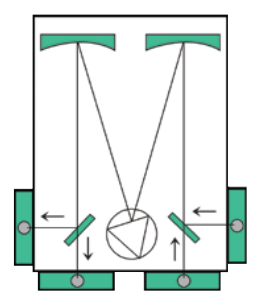
\includegraphics[width=3cm]{../results/spectrograph_sketch.png}
      \caption{}
  \end{subfigure}
  \hfill
  \begin{subfigure}[b]{6cm}
      \centering
      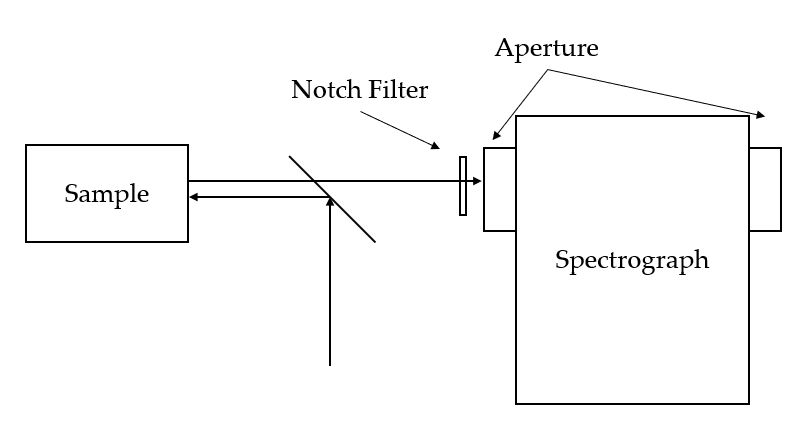
\includegraphics[width=6cm]{../results/total_module_sketch.png}
      \caption{}
  \end{subfigure}
  \hfill
  \caption{Schematic diagram of (a) spectrograph, adapted form  \cite{spectrograph_spec} (b)total photoluminescence module}
  \label{fig:apparatus_sketch}
\end{figure}


\subsection{Ruby : PL by temperature}
 I fix the alignment and set the sample pressure under 10mTorr using rotary pump.
 Then using compressor, lower the sample temperature from $270K$ to $10K$.
 If the grating speed is too fast, turn on the heater attached to sample to mediate the speed.
 I detect photons from CCD camera for every $5K$, and read the middle temperature of detection while proceeding.
 In this experiment, about $0.2K$ has cooled so the photoluminescence by temperature detection is vouched by accuracy of $0.1K$.


\section{Results and Discussion}\

All of the results are uploaded at \cite{github_results}.
In this report some sample plots are attatched, which does not influence generality of logical flows.
The file name and detailed contents are table at Fig. \ref{fig:file_appendix}

\begin{figure}[H]
  \centering
  \begin{tabular}{|c| c|}
      file name  & details \\
      \hline
      \verb|Ruby sx-y_raw_fig.png| & Ruby PL plot of slit width $x$ in repeated index $y$\\
      \verb|R6G(x)_raw_fig.png| & R6G PL plot of repeated index $x$, raw figure\\
      \verb|R6G(x)_gaussian_fitted_fig.png| & R6G PL plot of repeated index $x$ gaussian fitted figure\\
      \verb|Ruby(T)_raw_fig.png| & Ruby PL plot in temperature $T$ , raw  figure\\
      \verb|Ruby(T)_voigt_fitted_fig.png| & Ruby PL plot in temperature $T$, voigt fitted figure\\
      \verb|R6G_total_fig.png| & United plot of R6G sample\\
      \verb|Ruby_temperature_peak_fig.png| & United plot of Ruby sample, peak position statics\\
      \verb|Ruby_temperature_width_fig.png| & United plot of Ruby sample, peak width statics\\

  \end{tabular}
  \caption{file appendix of \cite{github_results}}
  \label{fig:file_appendix}
\end{figure}

\subsection{Aperture setting}
\label{result:aperture_effect}
 I repeatly measure ruby sample in same temperature, pressure and alignment condition, only changing the aperture slit width.
 Fig. \ref{fig:s5_s30_difference} shows two extreme case of $0.05 mm$ and $0.30 mm$ opened results.
 As the aperture closed, less photon are detected, the peaks doesn't dominate the results.
 But, the widely opened aperture makes resolution worse.
 In this trade off we choosed to take slit width of $0.25 mm$, since the Stokes sideband are significantly observable from that width.
 Which leads us to expect the minor band can be visable through the noise either.
 

 \begin{figure}[ht]
  \centering
  \begin{subfigure}[b]{6cm}
      \centering
      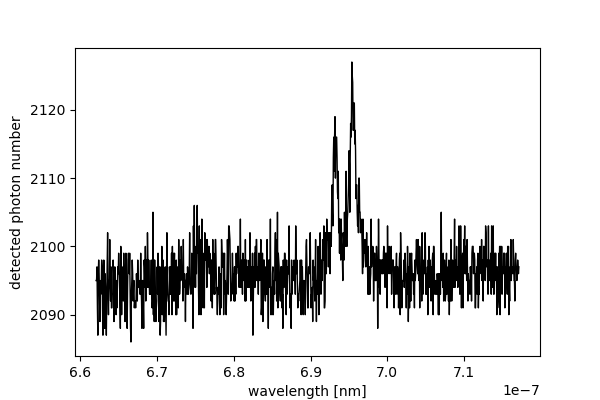
\includegraphics[width=6cm]{../results/Ruby s5-1_raw_fig.png}
      \caption{}
  \end{subfigure}
  \hfill
  \begin{subfigure}[b]{6cm}
      \centering
      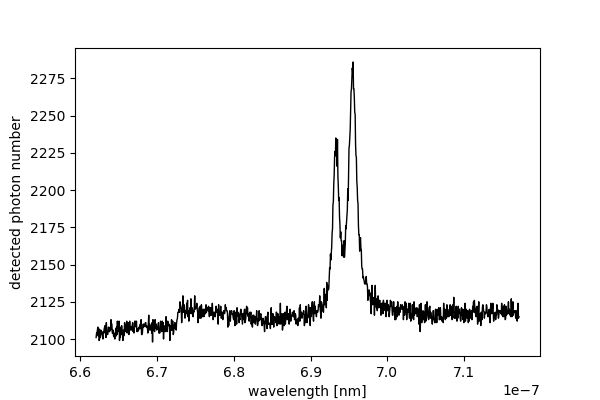
\includegraphics[width=6cm]{../results/Ruby s30-1_raw_fig.png}
      \caption{}
  \end{subfigure}
  \hfill
  \caption{PL result of ruby in (a)0.05mm (b)0.30mm opened aperture}
  \label{fig:s5_s30_difference}
\end{figure}
 
\subsection{Rhodamin 6G}
 Fig. \ref{fig:R6G results}(b) shows counts - energy [$eV$] plot and its gaussian trend line.
 Peak statics of five repeated detection is provided at Fig. \ref{fig:R6G optimize results}.
 $N(E) = A \frac{1} {\sigma \sqrt{2\pi}} e^{-\frac{1}{2} \frac{(E-E_0)^2}{\sigma^2}}$ values are obtained.
 The amplitude $A$ and background light $C$ does not inform a critical phenomena for R6G, the peak position and FWHM matters.
 The band gap betwen LUMO and HOMO is $2.211 \pm 0.001$ [$eV$] and its lifetime is $7.15 \pm 10^-15 $[$s$].
 \begin{figure}[ht]
  \centering
  \begin{subfigure}[b]{6cm}
      \centering
      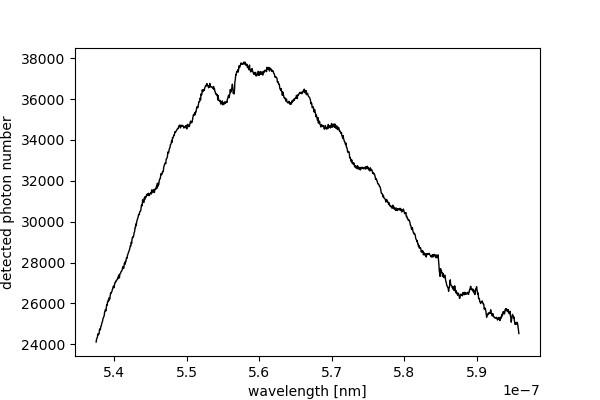
\includegraphics[width=6cm]{../results/R6G(1)_raw_fig.png}
      \caption{}
  \end{subfigure}
  \hfill
  \begin{subfigure}[b]{6cm}
      \centering
      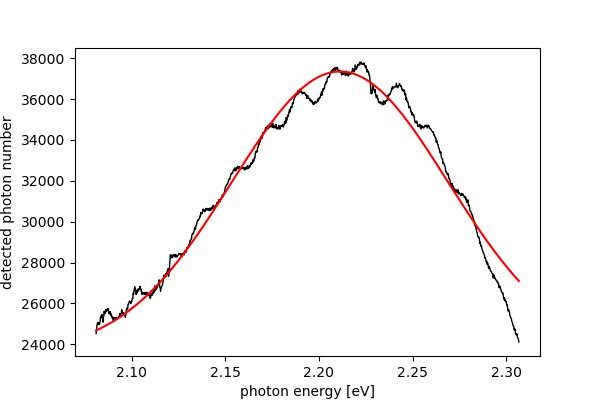
\includegraphics[width=6cm]{../results/R6G(1)_gaussian_fitted_fig.png}
      \caption{}
  \end{subfigure}
  \hfill
  \caption{PL result of R6G (a)counts - wavelength[$nm$] (b)counts - photon energy[$eV$]}
  \label{fig:R6G results}
\end{figure}

\begin{figure}[H]
  \centering
  \begin{tabular}{|c| c| c|c|c|}
      index  & $E_0 $[$eV$]  & $\sigma$ [$eV$] & $A$ & $C$\\
      \hline
      1 & $2.211$ & $5.78\times 10^{-2}$ & $1.99 \times 10^3$ & $2.36 \times 10^4$\\
      2 & $2.211$ & $5.77\times 10^{-2}$ & $2.10 \times 10^3$ & $2.47 \times 10^4$\\
      3 & $2.211$ & $5.77\times 10^{-2}$ & $1.92 \times 10^3$ & $2.30 \times 10^4$\\
      4 & $2.211$ & $5.77\times 10^{-2}$ & $2.03 \times 10^3$ & $2.41 \times 10^4$\\
      5 & $2.211$ & $5.76\times 10^{-2}$ & $2.06 \times 10^3$ & $2.45 \times 10^4$\\
      
  \end{tabular}
  \caption{Statics of Gaussian fitting of Fig. \ref{fig:R6G results} in different trials}
  \label{fig:R6G optimize results}
\end{figure}

The bumps on the peak is not a random error, but keep appears in repeated measurements.
Fig. \ref{fig:R6G total fig}(a) is the total plot of every datum in one plot.
We can check that exactly same sidebands are at same position in different experiments.
I have rotated the vials and moved the solutions position during the experiment, it does not have relation with outer variables.
Therefore, I assumes those sideband have relation with Raman scattering.
The Raman shift of R6G has calculated in \cite{rhodamine_HOMO_LUMO}.
As the molecule in solution moves freely in ethylene glycol, the cross section of the band gap might Raman shifted.
There are around 10~12 big peaks on raman shift as shown in Fig. \ref{fig:R6G total fig}(b), which is exactly same values to the experimental data.
Also, the dimer effect has reported from \cite{Rhodamine_dimer}, but in this experiment the solution is diluted enough to ignore the dimer effects.

 \begin{figure}[ht]
  \centering
  \begin{subfigure}[b]{6cm}
      \centering
      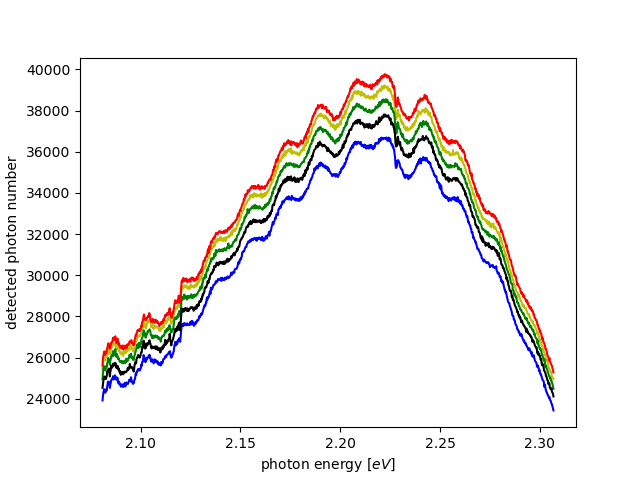
\includegraphics[width=6cm]{../results/R6G_total_fig.png}
      \caption{}
  \end{subfigure}
  \hfill
  \begin{subfigure}[b]{6cm}
      \centering
      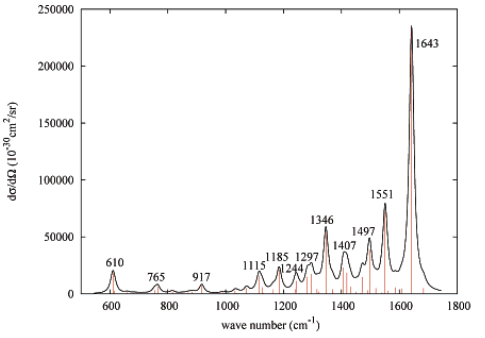
\includegraphics[width=6cm]{../results/Raman_shift.png}
      \caption{}
  \end{subfigure}
  \hfill
  \caption{(a)United plot of R6G PL data each color are the repeated measurements. (b)Raman shift calculation adapted from \cite{rhodamine_HOMO_LUMO}}
  \label{fig:R6G total fig}
\end{figure}


\subsection{Ruby PL result by temperature}
\label{result:temperature_peak_statics}  




\section{Summary}

\bibliography{photoluminescence_ref}
\bibliographystyle{plain}
\end{document}